% Original book diagram: fig:slam_loop_closure
% Book source: sections/Part_V/slam.tex
% Original diagram authorship retained. Visual design: Ziad Mosalam.
\documentclass[11pt,border=8pt]{standalone}
\usepackage{amsmath,amssymb,graphicx,tikz}
\usetikzlibrary{arrows.meta,automata,positioning,calc,shapes.geometric,fit,backgrounds,patterns}
\newcommand{\vect}[1]{\mathbf{#1}}
\newcommand{\mat}[1]{\mathbf{#1}}
\newcommand{\Normal}{\mathcal{N}}
\newcommand{\prob}{p}
\newcommand{\E}{\mathbb{E}}
\newcommand{\Var}{\mathrm{Var}}
\newcommand{\Cov}{\mathrm{Cov}}
\newcommand{\CovP}{\mathbf{P}}
\newcommand{\Prob}{\mathbb{P}}
\setlength{\textwidth}{6.5in}
% Shared visual vocabulary for the book's original diagrams.
% Figures opt in explicitly, so unrelated text and existing additions are unchanged.
\definecolor{BookBlue}{HTML}{003262}
\definecolor{BookGold}{HTML}{B17A00}
\definecolor{BookTeal}{HTML}{247C86}
\definecolor{BookInk}{HTML}{30363B}
\definecolor{BookLight}{HTML}{E9EFF5}
\tikzset{
  book figure/.style={font=\small\rmfamily, color=BookBlue, text=BookInk,
    line width=0.8pt, >=Latex},
  book axis/.style={->, draw=BookInk, line width=0.6pt},
  book link/.style={->, draw=BookBlue, line width=0.8pt},
  book observation/.style={draw=BookGold, fill=BookGold!8},
  book state/.style={draw=BookBlue, fill=BookLight},
  book note/.style={font=\footnotesize\rmfamily, text=BookInk}
}

\begin{document}
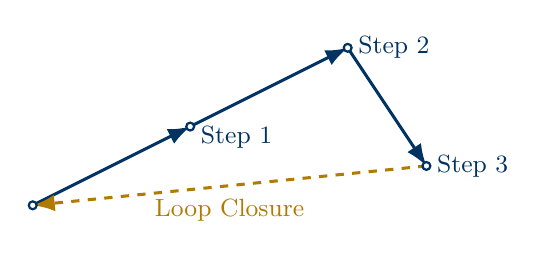
\begin{tikzpicture}[book figure, scale=1.0]
    \draw[BookBlue,line width=1.1pt,->] (0,0) -- (2,1) node[right, yshift=-4] {\small Step 1};
    \draw[BookBlue,line width=1.1pt,->] (2,1) -- (4,2) node[right] {\small Step 2};
    \draw[BookBlue,line width=1.1pt,->] (4,2) -- (5,0.5) node[right] {\small Step 3};
    \draw[BookGold,line width=1.1pt,->,dashed] (5,0.5) -- (0,0) node[midway,below, yshift=-1] {\small Loop Closure};
    \filldraw[fill=white,draw=BookBlue,line width=0.8pt] (0,0) circle (0.05);
    \filldraw[fill=white,draw=BookBlue,line width=0.8pt] (2,1) circle (0.05);
    \filldraw[fill=white,draw=BookBlue,line width=0.8pt] (4,2) circle (0.05);
    \filldraw[fill=white,draw=BookBlue,line width=0.8pt] (5,0.5) circle (0.05);
\end{tikzpicture}
\end{document}
